% !TEX root = batteryposter.tex

\documentclass[tikz]{standalone}
% !TEX root = batteryposter.tex

\usepackage{mwe}
\usepackage{blindtext}
\usepackage{relsize}
\usetikzlibrary{positioning	}
\usetikzlibrary{arrows.meta}
% Macros
\newcommand{\xo}{\bigotimes}

%%%%%%%%%%%%%%%%%%%%%%%%%%%%%%%%%%%%%%%%%%%%%%%%%%%%%%%%%%%%%%%%%%%%%%%%%%%%%%%%%%%%%%%%
% Poster parameters %%%%%%%%%%%%%%%%%%%%%%%%%%%%%%%%%%%%%%%%%%%%%%%%%%%%%%%%%%%%%%%%%%%%
%%%%%%%%%%%%%%%%%%%%%%%%%%%%%%%%%%%%%%%%%%%%%%%%%%%%%%%%%%%%%%%%%%%%%%%%%%%%%%%%%%%%%%%%

% Colours
\newcommand{\macrocolor}{red}
\newcommand{\microcolor}{blue}
\newcommand{\macrotext}[1]{\color{\macrocolor}#1}
\newcommand{\microtext}[1]{\color{\microcolor}#1}

% Graph box parameters
\newcommand{\FIGWIDTH}{14cm} % figure width
\newcommand{\FIGHEIGHT}{9cm} % figure height
\newcommand{\VERTFIGSEP}{5cm} % vertical separation between figures
\newcommand{\HORFIGSEP}{7cm} % horizontal separation between figures

% Axis box and line style
\tikzstyle{axisbox} = [inner sep=0]
\tikzstyle{axisline} = [
		% {Latex[length=1cm, width=1cm]}-{Latex[length=1cm, width=1cm]},
		-{Latex[length=1cm, width=1cm]},
		ultra thick,
		>=stealth
]

% Model point style
\tikzstyle{modelpoint} = [
		circle,
		fill=black,
		inner sep=0pt,
		minimum size=0.5cm,
		% prefix after command= {\pgfextra{\tikzset{every label/.style={font=\Huge}}}}
]

% Textbox style
\tikzstyle{mybox} = [
		draw=red,
		fill=blue!20,
		very thick,
    rectangle,
		rounded corners,
		inner sep=10pt,
		inner ysep=20pt]
\tikzstyle{fancytitle} = [fill=red, text=white]

%%%%%%%%%%%%%%%%%%%%%%%%%%%%%%%%%%%%%%%%%%%%%%%%%%%%%%%%%%%%%%%%%%%%%%%%%%%%%%%%%%%%%%%%
%%%%%%%%%%%%%%%%%%%%%%%%%%%%%%%%%%%%%%%%%%%%%%%%%%%%%%%%%%%%%%%%%%%%%%%%%%%%%%%%%%%%%%%%

\usepackage[utf8]{inputenc}
\usepackage[T1]{fontenc}
\usepackage{libertine}
\usepackage[libertine]{newtxmath}

\usepackage{shellesc}

\usepackage{siunitx}


\usepackage{pgfplots}
%\usepackage{pgfplotstable}
\usepgfplotslibrary{colormaps}
%\usepackage[caption=false]{subfig}
\usepackage{subcaption}
\usepackage{graphicx, floatrow}

\usepackage{lipsum}

\usetikzlibrary{backgrounds}

%
%usepackage{pgf}
%usepackage{mathtools}
\pgfplotsset{compat=newest}

%\usepackage{tikz}
%\usetikzlibrary{external}
%\tikzexternalize % activate!

\definecolor{c1}{RGB}{228,26,28}
\definecolor{c2}{RGB}{55,126,184}
\definecolor{c3}{RGB}{77,175,74}
\definecolor{c4}{RGB}{152,78,163}
\definecolor{c5}{RGB}{255,127,0}
\definecolor{c6}{RGB}{106,61,154}



%\usefonttheme[onlymath]{serif}


\newcommand{\PLOTLINES}{0.7mm}
\newcommand{\AXISLINEWIDTH}{0.7mm}


\pgfplotscreateplotcyclelist{mylist}{
{c1, line width=\PLOTLINES},
{c2,line width=\PLOTLINES},
{c3,line width=\PLOTLINES},
{c4,line width=\PLOTLINES},
{c5,line width=\PLOTLINES},
{c1,dashed,line width=\PLOTLINES},
{c1,dotted,line width=\PLOTLINES},
{c2,dashed,line width=\PLOTLINES},
{c2,dotted,line width=\PLOTLINES},
{c3,dashed,line width=\PLOTLINES},
{c3,dotted,line width=\PLOTLINES},
{c4,dashed,line width=\PLOTLINES},
{c4,dotted,line width=\PLOTLINES},
{c5,dashed,line width=\PLOTLINES},
{c5,dotted,line width=\PLOTLINES}}


\newenvironment{customlegend}[1][]{%
    \begingroup
    % inits/clears the lists (which might be populated from previous
    % axes):
    \csname pgfplots@init@cleared@structures\endcsname
    \pgfplotsset{#1}%
}{%
    % draws the legend:
    \csname pgfplots@createlegend\endcsname
    \endgroup
}%

% makes \addlegendimage available (typically only available within an
% axis environment):
\def\addlegendimage{\csname pgfplots@addlegendimage\endcsname}
\usepackage{mhchem}
\usepackage{siunitx}
\DeclareSIUnit\Molar{\textsc{m}}

\usepackage{standalone}

\begin{document}
\begin{tikzpicture}
	% Grid lines (comment out to turn off)
	% \draw[help lines,color=black,xstep=1,ystep=1] (0,0) grid (80,90);
	% \foreach \x in {0,1,...,24} { \node [anchor=north] at (\x,0) {\x}; }
	% \foreach \y in {0,1,...,29} { \node [anchor=east] at (0,\y) {\y}; }

	% Full 3D
	% \node [axisbox, anchor=north west](3d_full) at (0,90) {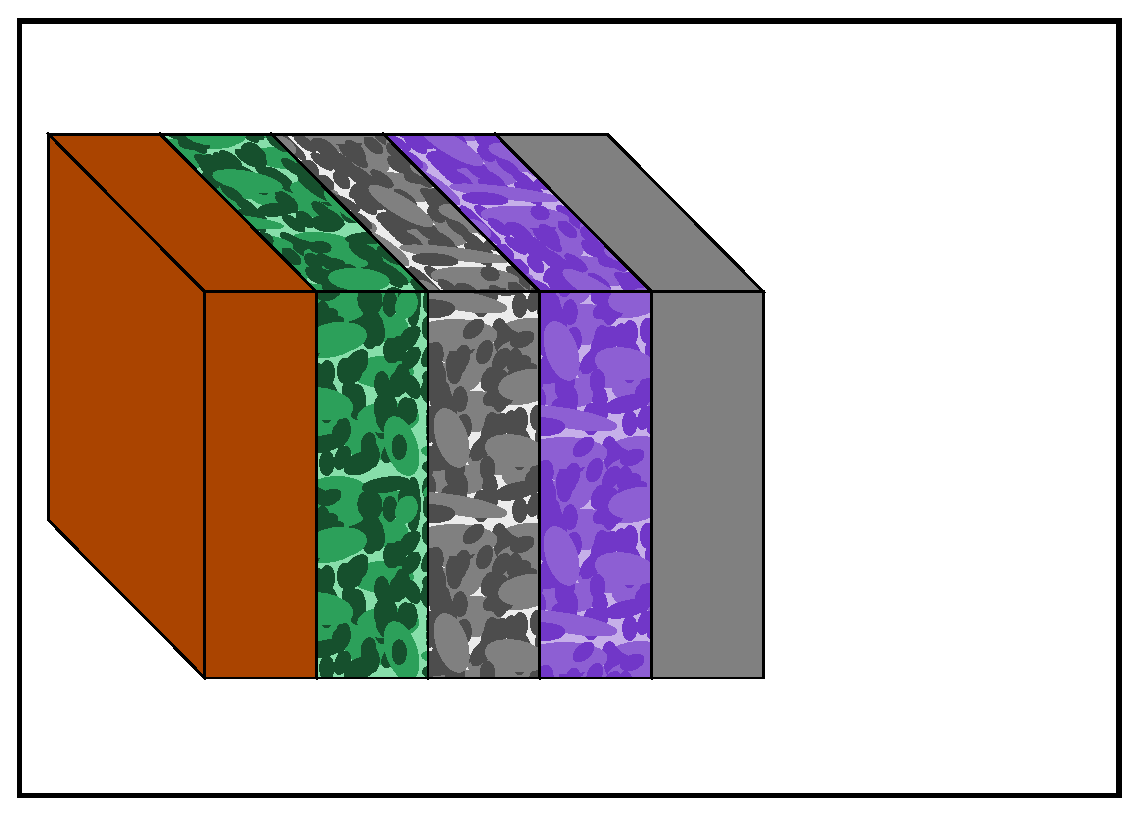
\includegraphics[width=\FIGWIDTH, height=\FIGHEIGHT]{figures/3D_unhomogenised}};

	% % Text
	% \node[textboxtitle,  above right = 0cm and 3cm of 3d_full, anchor=north west]
	% 	(title) {Introduction};
	% \node [textbox, anchor=north west] (box) at (title.south west) {%
	% 	\begin{minipage}{0.75\textwidth}
	% 			\blinditemize[4]
	% 	\end{minipage}
	% };


	% 3 + 3
	% \node [axisbox, below = \VERTFIGSEP of 3d_full, anchor=north](3D_homogenised_micro)
	% 	{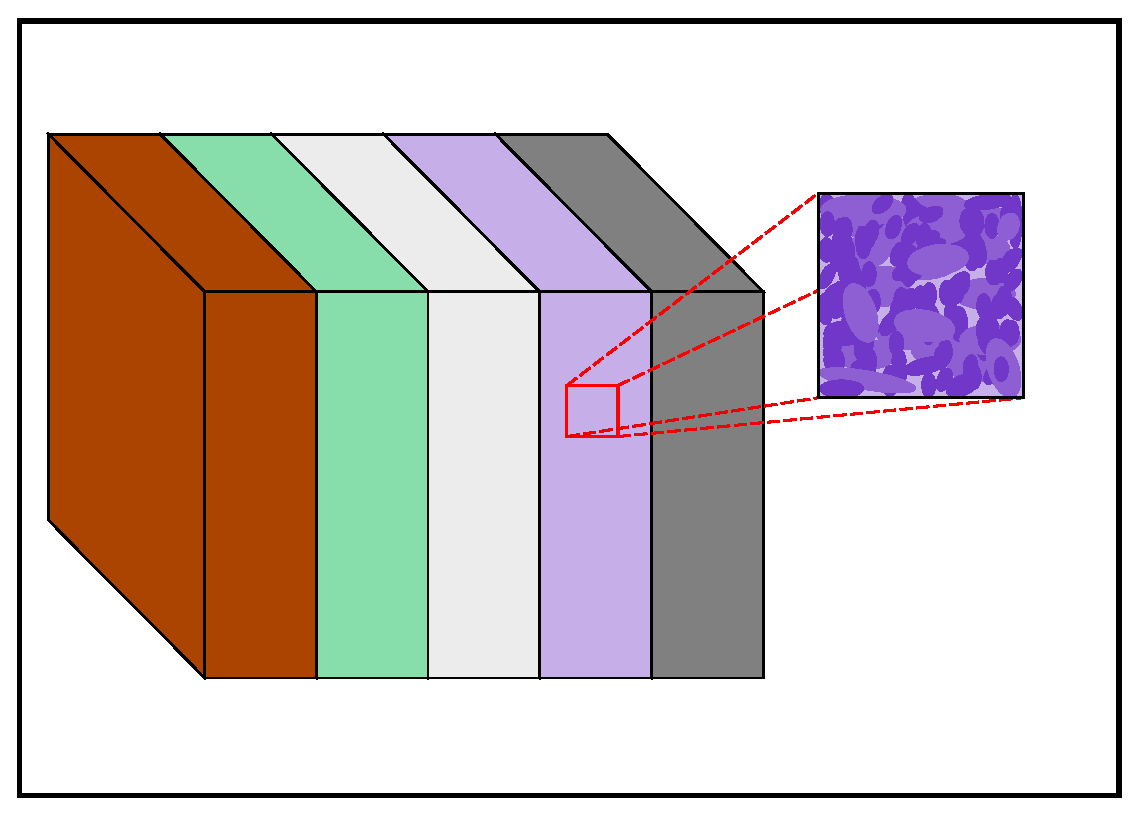
\includegraphics[width=\FIGWIDTH, height=\FIGHEIGHT]{figures/3D_homogenised_micro}};
	\node [axisbox, anchor=north west](3D_homogenised_micro) at (0,70) {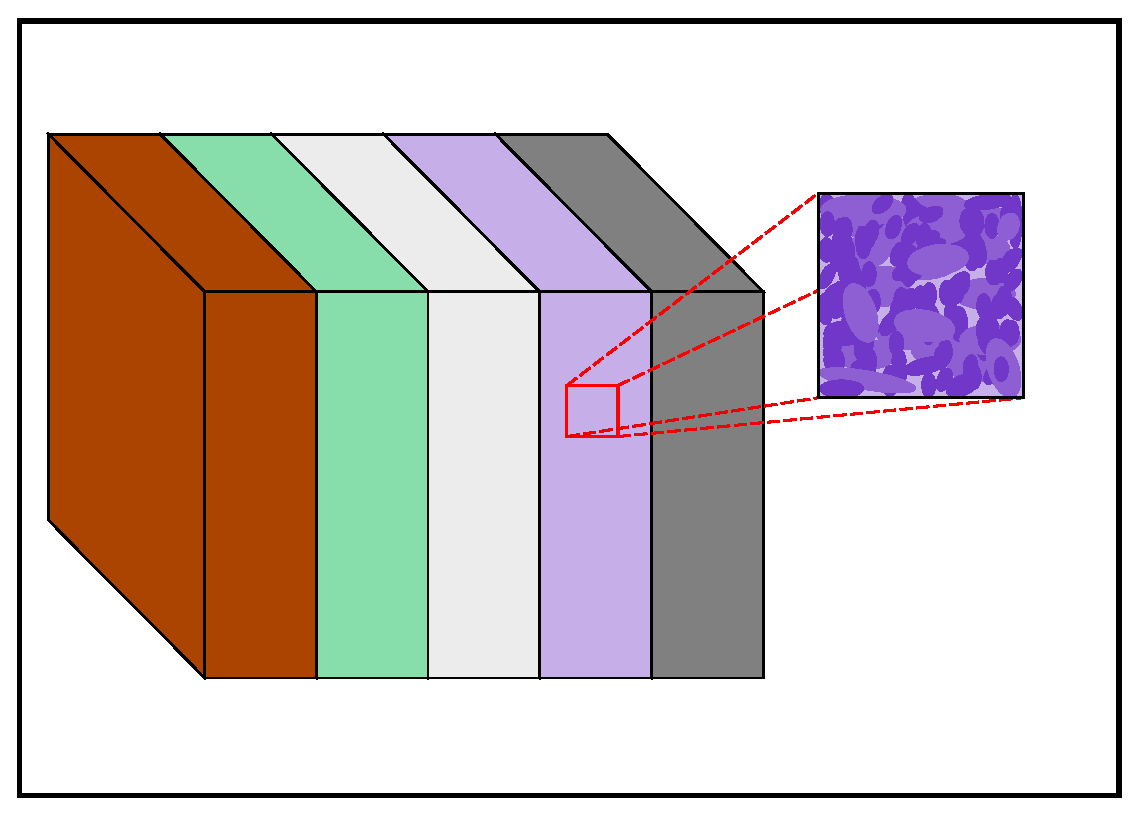
\includegraphics[width=\FIGWIDTH, height=\FIGHEIGHT]{figures/3D_homogenised_micro}};
	\draw [black, line width=\BORDERWIDTH]
		(3D_homogenised_micro.south west) rectangle (3D_homogenised_micro.north east);
	  \node [dimensions] at (3D_homogenised_micro.north east) {$\macrotext{(3)}\black{\xo}\microtext{(3)}$};
	\node [physics] at (3D_homogenised_micro.south east) {Full 3D};

	%
	% Microscale row and axis
	%
	\node [axisbox, microcolor, right = \HORFIGSEP of 3D_homogenised_micro, anchor=west]
		(particle_distribution)
		{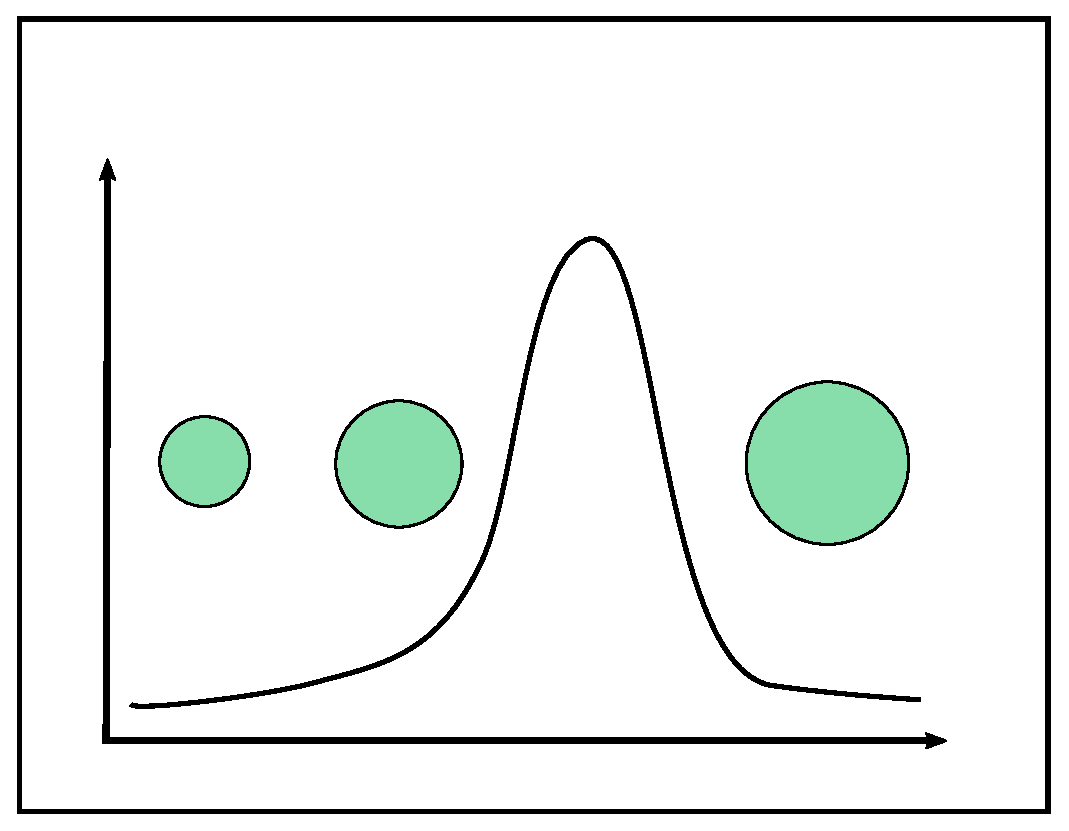
\includegraphics[width=\FIGWIDTH, height=\FIGHEIGHT]
			{figures/particle_distribution}};
	\draw [microcolor, line width=\BORDERWIDTH]
		(particle_distribution.south west) rectangle (particle_distribution.north east);
	  \node [dimensions] at (particle_distribution.north east) {$\macrotext{(\phantom{3})}\black{\xo}\microtext{(1\xo1)}$};
	\node [physics] at (particle_distribution.south east) {Spherical \\ particles};
	%
	\node [axisbox, microcolor, right = \HORFIGSEP of particle_distribution, anchor=west]
		(single_particle)
		{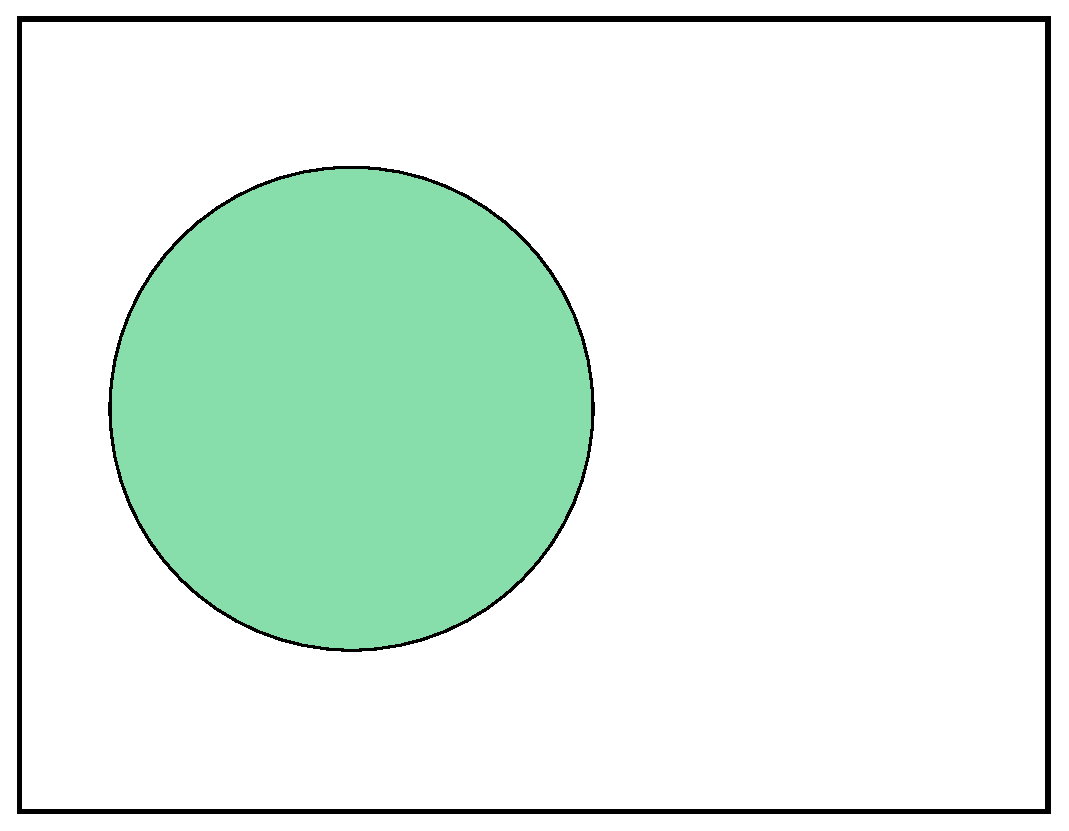
\includegraphics[width=\FIGWIDTH, height=\FIGHEIGHT]{figures/single_particle}};
	\draw [microcolor, line width=\BORDERWIDTH]
		(single_particle.south west) rectangle (single_particle.north east);
	\node [dimensions, microcolor] at (single_particle.north east) {$\macrotext{(\phantom{3})}\black{\xo}\microtext{(1)}$};
	\node [physics] at (single_particle.south east) {Narrow particle \\ distribution};
	%
	\node [axisbox, microcolor, right = \HORFIGSEP of single_particle, anchor=west](0D_micro)
		{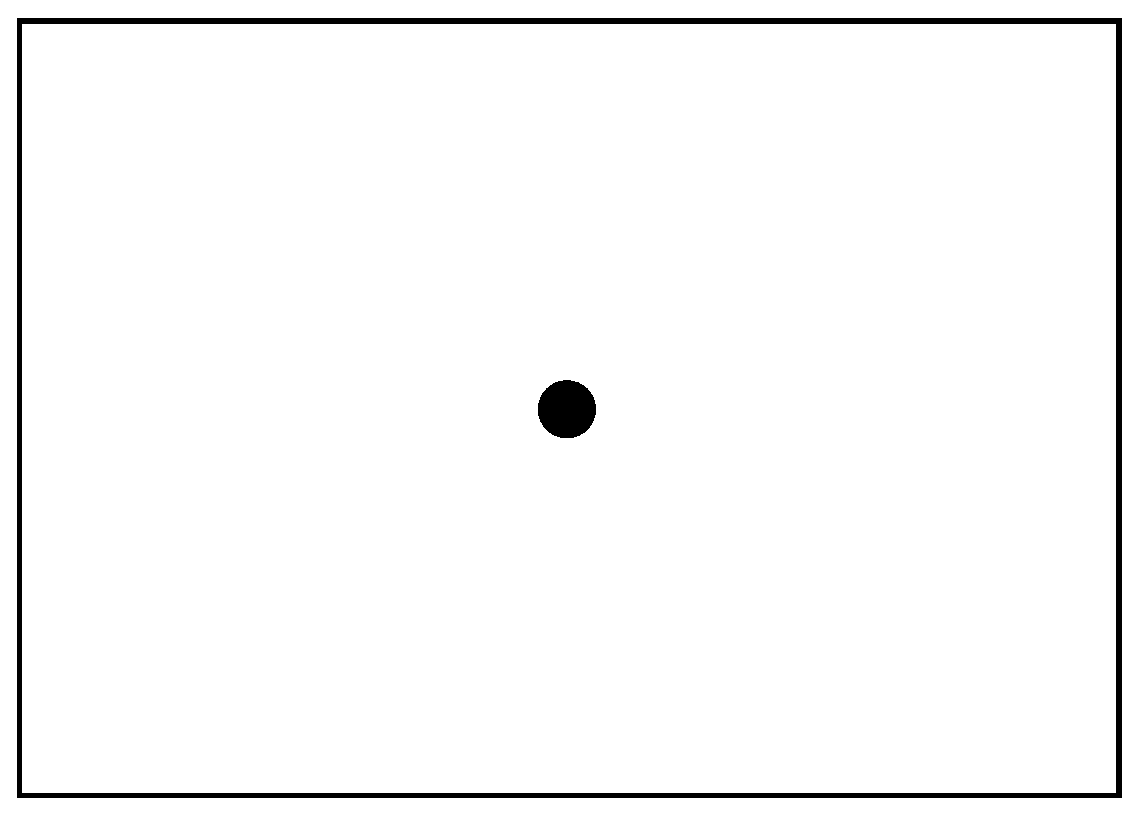
\includegraphics[width=\FIGWIDTH, height=\FIGHEIGHT]{figures/0D}};
	\draw [microcolor, line width=\BORDERWIDTH]
		(0D_micro.south west) rectangle (0D_micro.north east);
	\node [dimensions, microcolor] at (0D_micro.north east) {$\macrotext{(\phantom{3})}\black{\xo}\microtext{(0)}$};
	\node [physics] at (0D_micro.south east) {Fast diffusion \\ in particles};
	% axis
	% \node [below left = 3cm and 0cm of particle_distribution](x_axis_start) {};
	% \node [below right = 3cm and 0cm of 0D_micro](x_axis_end) {};
	\node [below right = 3cm and 3cm of 3D_homogenised_micro, anchor=center]
		(axis_origin) {$+$};
	\node (x_axis_end) at (axis_origin -| 0D_micro.east) {};
	\draw [axisline, microcolor] (axis_origin) -- (x_axis_end)
		node [above, pos=0, anchor=south west] {Complex}
		node [above, pos=0.5, anchor=south] {\Large \textsc{Microscale}}
		node [above, pos=1, anchor=south east] {Simple};
	%
	% Macroscale column
	%
	\node [axisbox, below = \VERTFIGSEP of 3D_homogenised_micro, anchor=north](2plus1D)
		{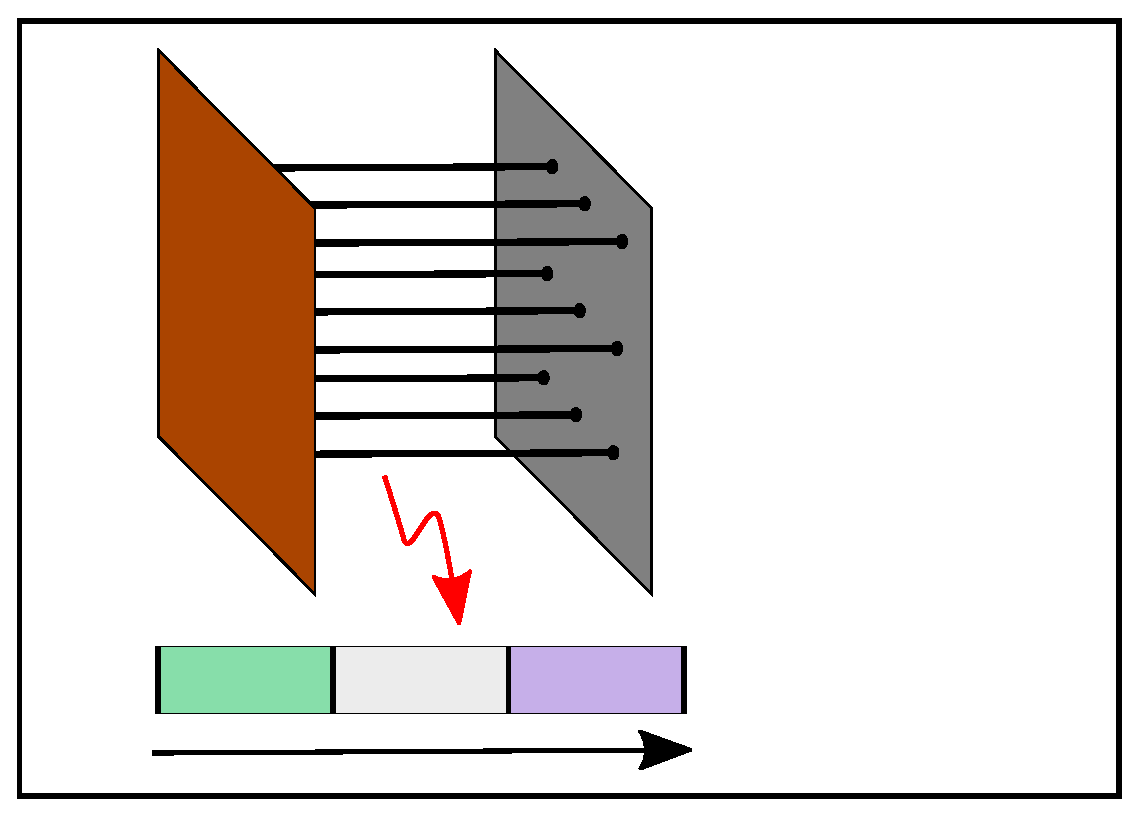
\includegraphics[width=\FIGWIDTH, height=\FIGHEIGHT]{figures/2plus1D}};
	\draw [macrocolor, line width=\BORDERWIDTH]
		(2plus1D.south west) rectangle (2plus1D.north east);
		\node [dimensions, macrocolor] at (2plus1D.north east) {$\macrotext{(2+1)}\black{\xo}\microtext{(\phantom{3})}$};
	\node [physics] at (2plus1D.south east) {Thin \\ electrodes};
	%
	\node [axisbox, below = \VERTFIGSEP of 2plus1D, anchor=north](2plusbar1D)
		{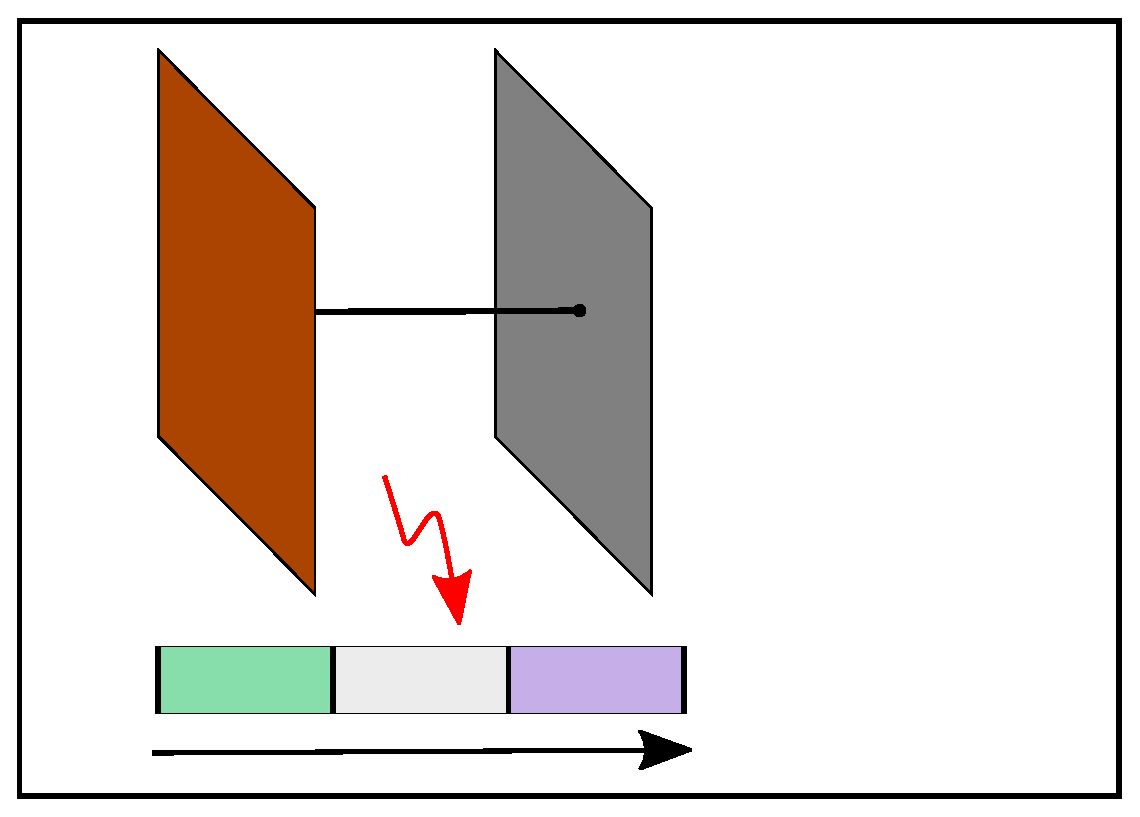
\includegraphics[width=\FIGWIDTH, height=\FIGHEIGHT]{figures/2plusbar1D}};
	\draw [macrocolor, line width=\BORDERWIDTH]
		(2plusbar1D.south west) rectangle (2plusbar1D.north east);
		\node [dimensions, macrocolor] at (2plusbar1D.north east) {$\macrotext{(2+\bar{1})}\black{\xo}\microtext{(\phantom{3})}$};
	\node [physics] at (2plusbar1D.south east) {Large \\ conductivity};
	%
	\node [axisbox, below = \VERTFIGSEP of 2plusbar1D, anchor=north](0plus1D)
		{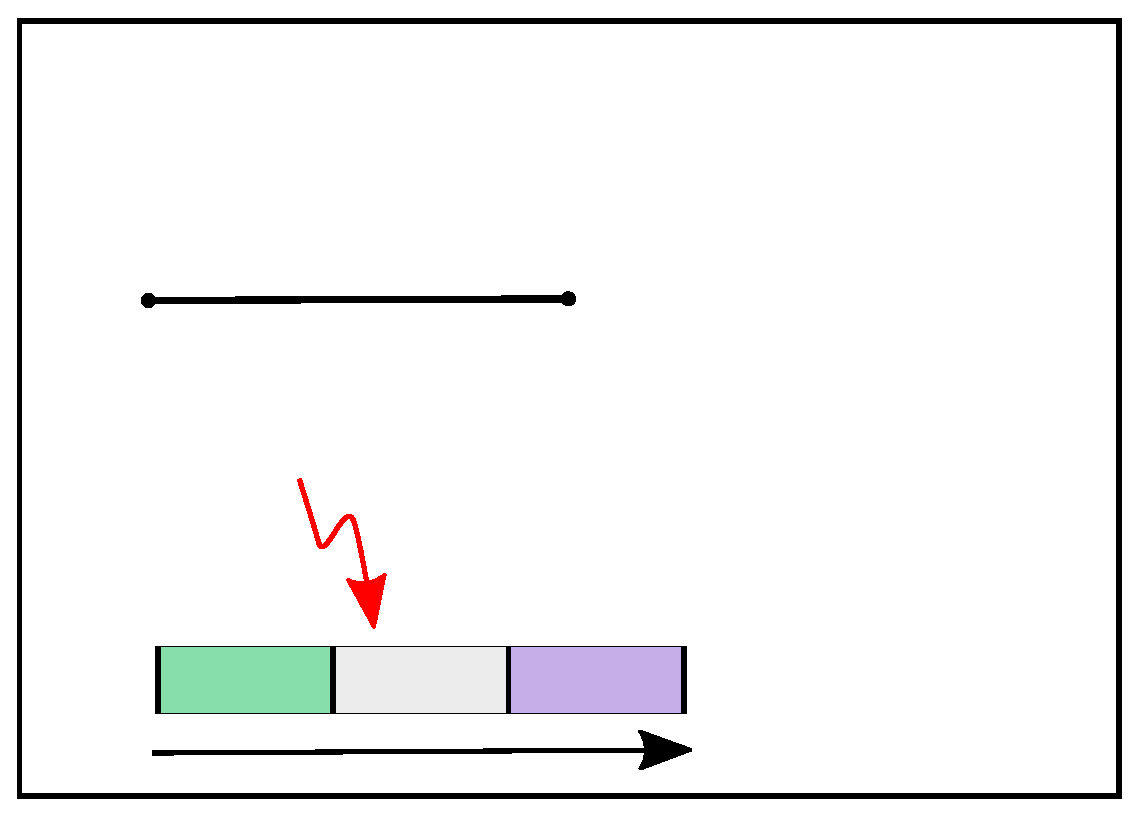
\includegraphics[width=\FIGWIDTH, height=\FIGHEIGHT]{figures/0plus1D}};
	\draw [macrocolor, line width=\BORDERWIDTH]
		(0plus1D.south west) rectangle (0plus1D.north east);
	\node [dimensions, macrocolor] at (0plus1D.north east) {$\macrotext{(1)}\black{\xo}\microtext{(\phantom{3})}$};
	\node [physics] at (0plus1D.south east) {Very large \\ conductivity};
	%
	\node [axisbox, below = \VERTFIGSEP of 0plus1D, anchor=north](0D_macro)
		{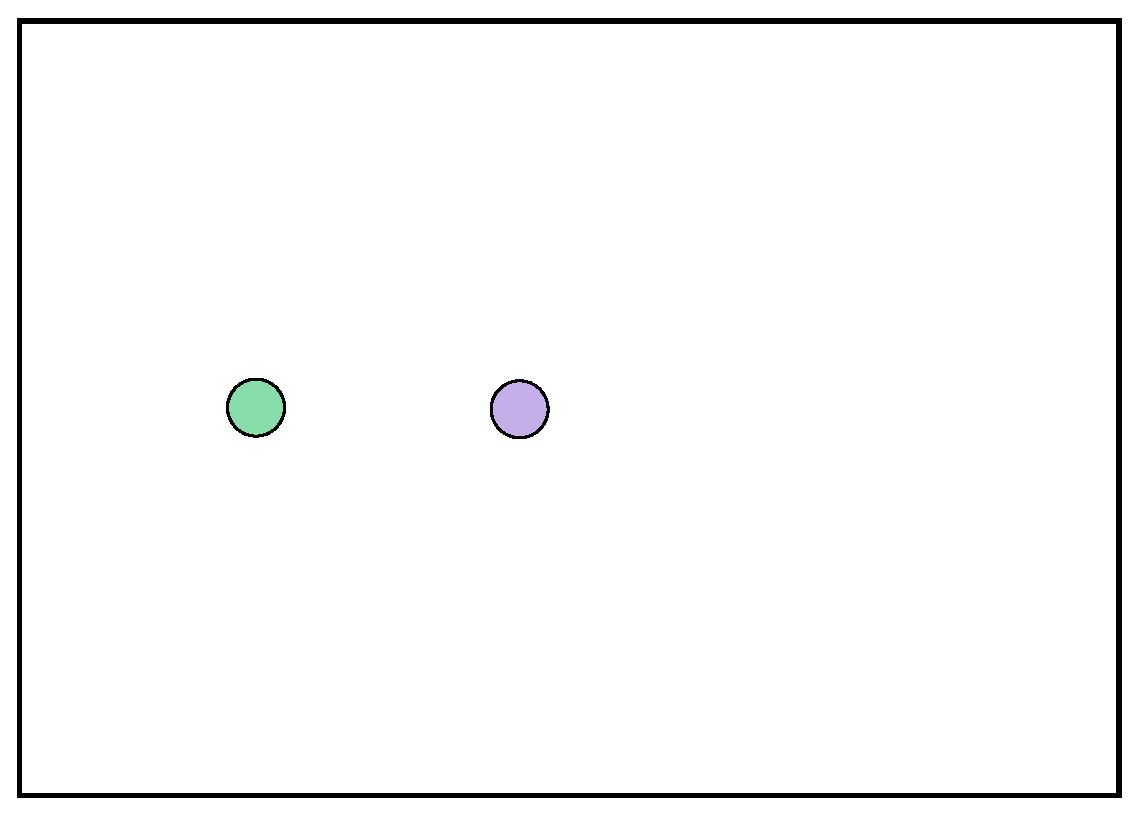
\includegraphics[width=\FIGWIDTH, height=\FIGHEIGHT]{figures/0D_macro}};
	\draw [macrocolor, line width=\BORDERWIDTH]
		(0D_macro.south west) rectangle (0D_macro.north east);
	\node [dimensions, macrocolor] at (0D_macro.north east) {$\macrotext{(0)}\black{\xo}\microtext{(\phantom{3})}$};
	\node [physics] at (0D_macro.south east) {Fast diffusion \\ in electrolyte};

	%%%%%%%%%%%%%%%%%%%%%%%%%%%%%%%%%%%%%%%%%%%%%%%%%%%%%%%%%%%%%%%%%%%%%%%%%%%%%%%%%%%%%%
	% Inner plot %%%%%%%%%%%%%%%%%%%%%%%%%%%%%%%%%%%%%%%%%%%%%%%%%%%%%%%%%%%%%%%%%%%%%%%%%
	%%%%%%%%%%%%%%%%%%%%%%%%%%%%%%%%%%%%%%%%%%%%%%%%%%%%%%%%%%%%%%%%%%%%%%%%%%%%%%%%%%%%%%
	%
	% 2D+1D models
	%
	\node [
		modelpoint,
		label=below:{
			RPPM \\[\labellinespace]
			{\tiny Reduced} \\[\labellinespace]
			{\tiny Potential} \\[\labellinespace]
			{\tiny Pair Model}
			}
	]
		 (2plus1D_0D) at ($(2plus1D -| 0D_micro)!0.8!(2plus1D -| 0D_micro.east)$) {};
	\node [
		modelpoint,
		label=right:{
			SPMeCC \\[\labellinespace]
			{\tiny Single Particle Model} \\[\labellinespace]
			{\tiny with Electrolyte and} \\[\labellinespace]
			{\tiny Current Collectors}
			}
	]
		(SPMeCC)
		at ($(2plusbar1D.north -| single_particle.west)!0.8!(2plusbar1D -| single_particle)$)
		{};
	\node [
		modelpoint,
		label=below:{ APPM \\[\labellinespace]
		  {\tiny Averaged} \\[\labellinespace]
		  {\tiny Potential} \\[\labellinespace]
		  {\tiny Pair Model}
		}
	]
		(2plusbar1D_0D) at (SPMeCC-| 2plus1D_0D) {};
	% Results
	\node [axisbox, fill=white, draw,line width=3mm, below left = 5cm and -1cm of particle_distribution, anchor=north west, minimum width=53.5cm,minimum height=14cm]
		(2D_results) {\hspace{1.5em} 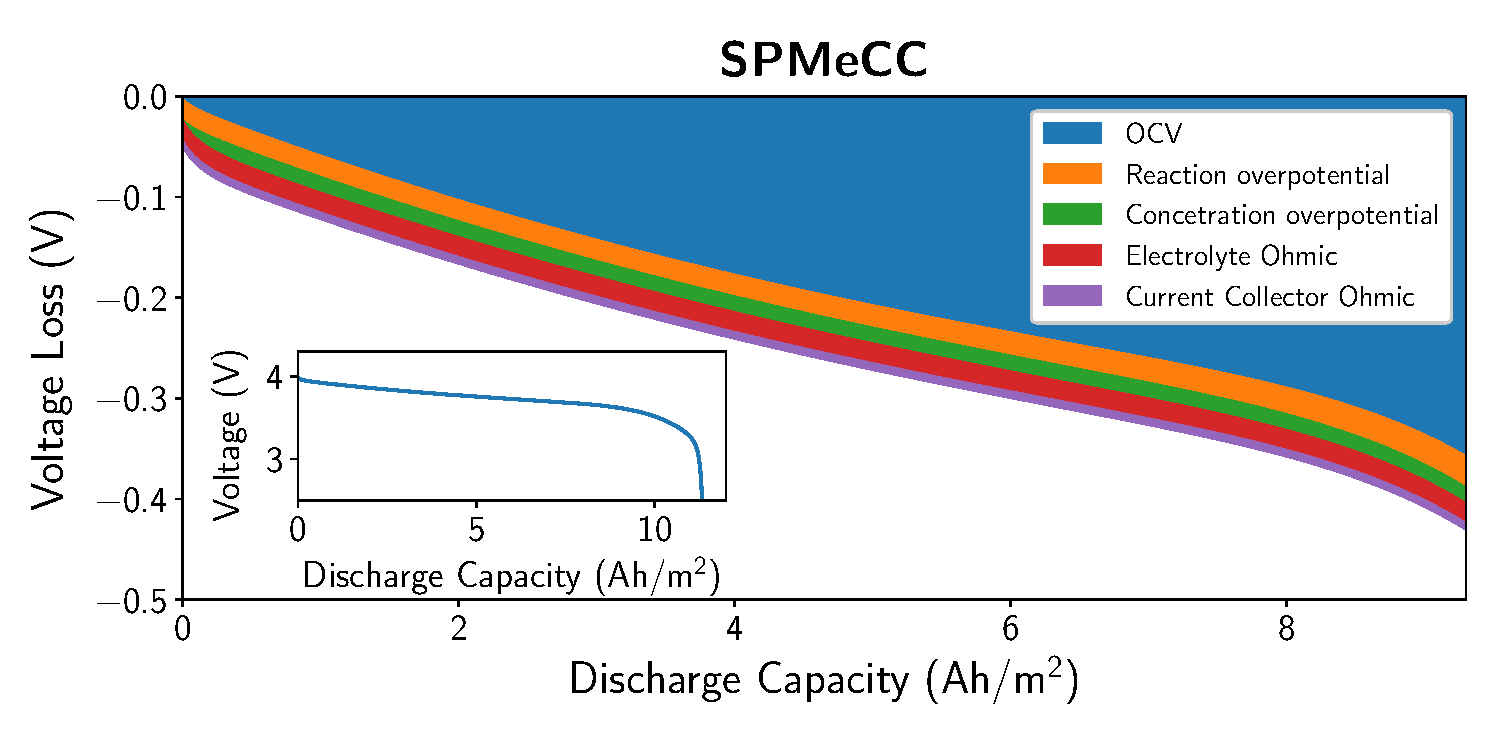
\includegraphics{figures/V_SPMeCC} 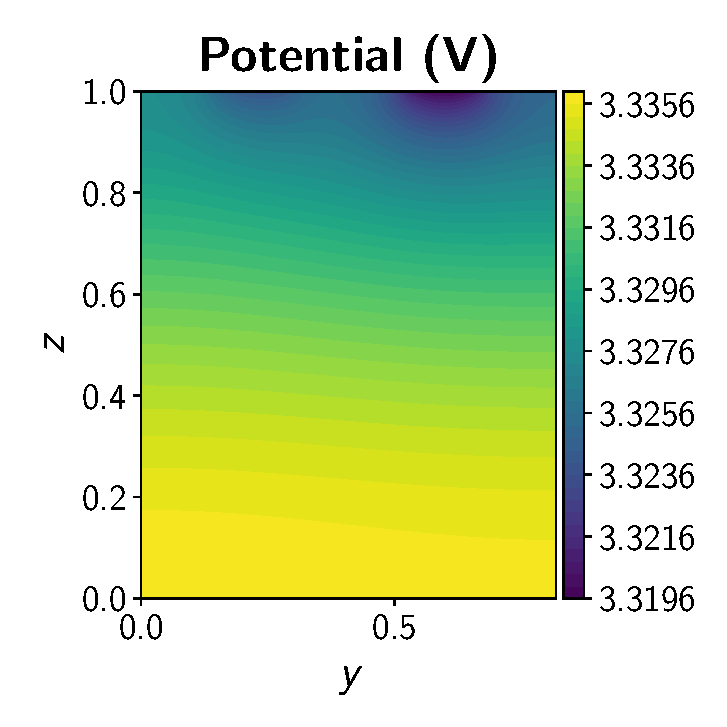
\includegraphics{figures/V_2D} 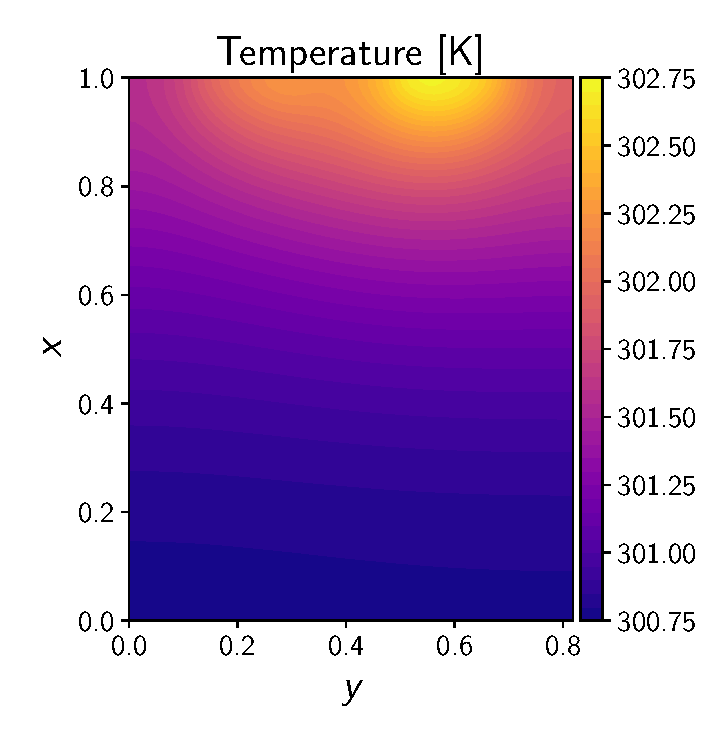
\includegraphics{figures/T_2D}};
	\node [anchor=north west, align=left, font=\small] (2D_title)
		at (2D_results.north west) {Lithium Cobalt Oxide};

	\picbox{images/portraits/sulzer.jpg}{tino_2D}{2D_results.south west}{south west}
	\picbox{images/portraits/ScottMarquis.png}{scott_2D}{tino_2D.north west}{south west}
	\picbox{images/portraits/rtimms_photo.jpg}{rob_2D}{scott_2D.north west}{south west}

	% Arrows
	\draw [results_arrow] (2plus1D_0D) -- (2plus1D_0D -| 2D_results.east);
	\draw [results_arrow] (SPMeCC) -- (2D_results.south -| SPMeCC);
	\draw [results_arrow] (2plusbar1D_0D) -- (2D_results.south east);

	%
	% DFN, SPMe, SPM
	%
	\node [
		modelpoint,
		label=right:{
			DFN \\[\labellinespace]
			{\tiny Doyle-Fuller-Newman}
		}
	]
		(DFN) at
		($(0plus1D.north -| SPMeCC)!0.5!(2plusbar1D.south -| SPMeCC)$) {};
	\node [
		modelpoint,
		label=right:{
		  SPM \\[\labellinespace] {\tiny Single Particle Model}
		}
	]
		(SPM)
		% at ($(0D_macro -| single_particle)!0.6!(0D_macro.north -| single_particle)$) {};
		at ($(0D_macro -| SPMeCC)!0.6!(0plus1D -| SPMeCC)$) {};
	\node [
		modelpoint,
		label=right:{
			SPMe \\[\labellinespace]
			{\tiny Single Particle Model} \\[\labellinespace]
			{\tiny with Electrolyte}
		}
	]
		(SPMe) at ($(SPM)!0.5!(DFN)$) {};
	% Results
	\node [axisbox, below left = 1.5cm and 0cm of 2D_results, anchor=north west]
	(SPM_results) {\includestandalone[width=25cm, height=24cm]{plot_SPM}};
	\node [anchor=north west, align=left, font=\small] (2D_title)
		at (SPM_results.north west) {Lithium Cobalt Oxide};
	\picbox{images/portraits/rtimms_photo.jpg}{rob_SPM}{SPM_results.south east}{south east}
	\picbox{images/portraits/ScottMarquis.png}{scott_SPM}{rob_SPM.south west}{south east}

	% Arrows
	\draw [results_arrow] (DFN) -- (DFN -| SPM_results.east);
	\draw [results_arrow] (SPMe) -- (SPMe -| SPM_results.east);
	\draw [results_arrow] (SPM) -- (SPM_results.south east);

	%
	% Distributed Particle Models
	%
	\node [
		modelpoint,
		label=right:{
				DPM \\[\labellinespace] {\tiny Distributed Particle Model}
			}
	]
		(DPM) at (SPM -| particle_distribution) {};
	\node [
		modelpoint,
		label=right:{
			MPM \\[\labellinespace]
			{\tiny Multiple Particle Model}
		}
	]
		(MPM) at ($(SPM)!0.5!(DPM)$) {};
	% Results
	\node [axisbox, fill=white, draw, line width=3mm, anchor=north west, minimum width=33cm,minimum height=17cm] (distributed_results)
		at ($(0D_macro.north-| SPM_results.west)!0.5!(DPM-| SPM_results.west)$)
		{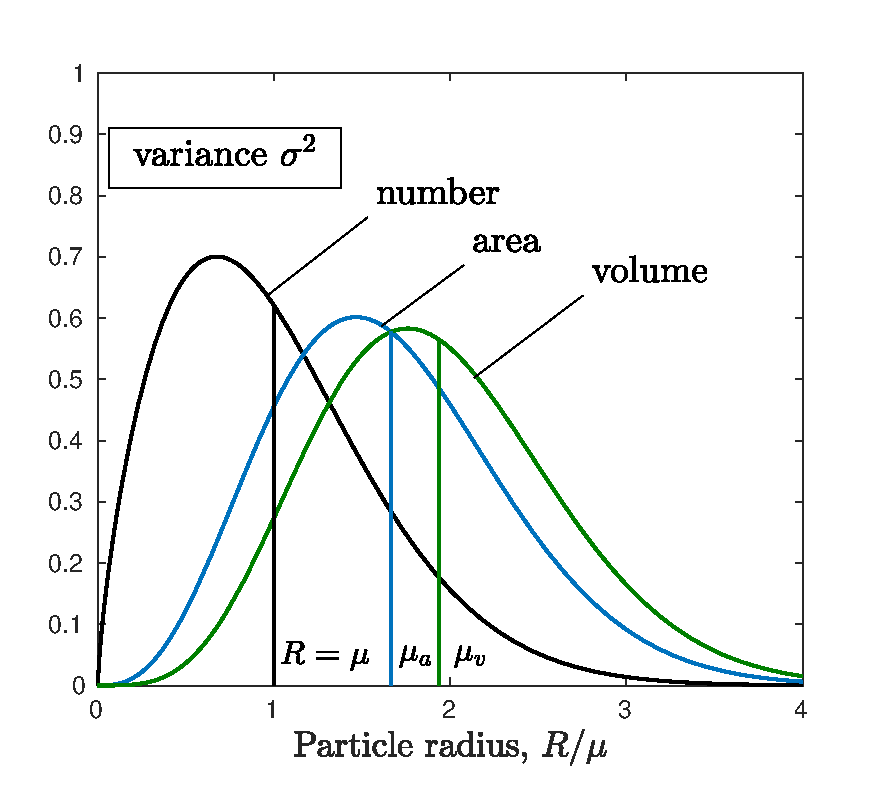
\includegraphics[height=14.5cm]{figures/PSD_results_1}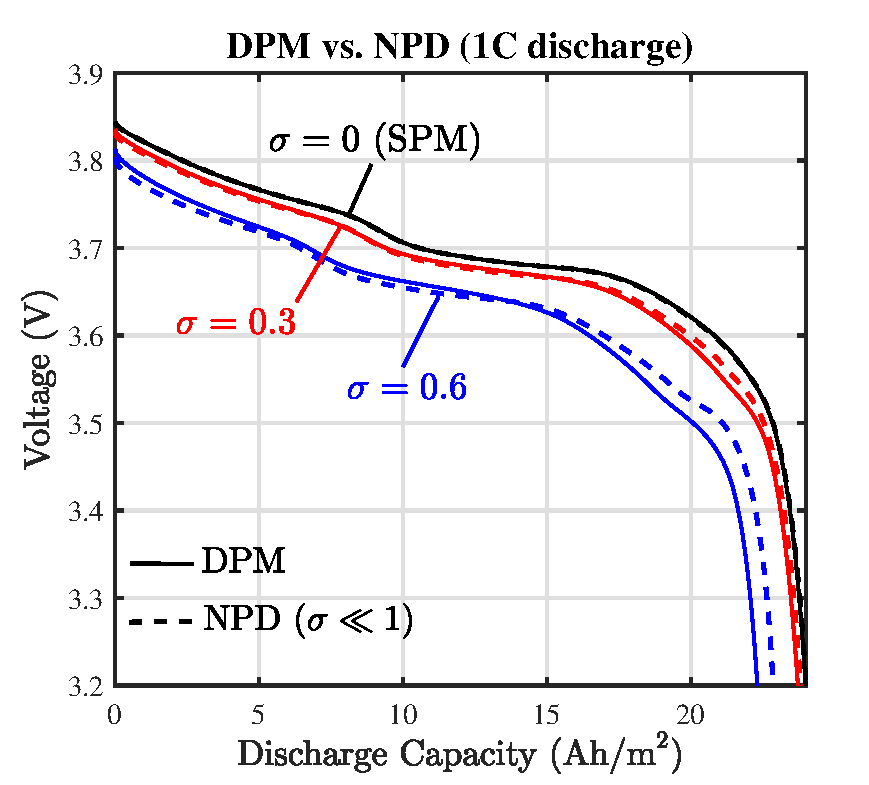
\includegraphics[height=14.5cm]{figures/PSD_results_2}};
	\node [anchor=north west, align=left, font=\small] (2D_title)
		at (distributed_results.north west) {Lithium Cobalt Oxide};
	\picbox{images/portraits/tobykirk_photo.jpg}{toby}{distributed_results.south west}{south west}

	% Arrows
	\draw [results_arrow] (DPM) -- (distributed_results.north -| DPM);
	\draw [results_arrow] (MPM) -- (distributed_results.north -| MPM);
	\draw [results_arrow] (SPM) -- (distributed_results.north -| SPM);

	%
	% Fast diffusion models
	%
	\node [
		modelpoint,
		label=below:{NT \\[\labellinespace]
		  {\tiny Newman-} \\[\labellinespace]
			{\tiny Tiedemann}
		}
	]
		(DFNfast) at (DFN -| 2plus1D_0D) {};
	\node [
		modelpoint,
		label=below:{ODEM \\[\labellinespace]
	 	{\tiny Ordinary} \\[\labellinespace]
		{\tiny Differential} \\[\labellinespace]
		{\tiny Equation} \\[\labellinespace]
		{\tiny Model}
		}
	]
		(SPMfast) at (SPM -| 2plus1D_0D) {};
	\node [
		modelpoint,
		label=below:{FOQS \\[\labellinespace]
		  {\tiny First-Order} \\[\labellinespace]
		  {\tiny Quasi-Static} \\[\labellinespace]
		  {\tiny Model}
	  }
	]
		(SPMefast) at ($(SPMfast)!0.5!(DFNfast)$) {};
	% Results
	% make this a tikzstyle
	\node [axisbox, fill=white, draw,line width=3mm, right = 2cm of distributed_results.south east, anchor=south west,minimum width=18cm,minimum height=44.5cm] (fast_results) {};
	% lead-acid
	\node [anchor=north west] (lead_acid_title)
		at (fast_results.north west) {\small Lead-Acid};
	\picbox{images/portraits/sulzer.jpg}{tino_fast}{fast_results.north east}{north east}
	\node [anchor=north] (lead_acid)
		at (lead_acid_title.south -| fast_results.north)
		{\includestandalone[width=17cm]{plot_lead_acid}};
	%lifp
	\node (lifp_start) at ($(lead_acid.south) + (0,-1cm)$) {};
	\draw [line width=1mm]
		(lifp_start -| fast_results.west)
		-- (lifp_start -| fast_results.east);
	\node [anchor=north west] (lifp_title)
		at (lifp_start -| fast_results.west)
		{\small Lithium Iron Phosphate};
	\node [anchor=south] at (fast_results.south)
		{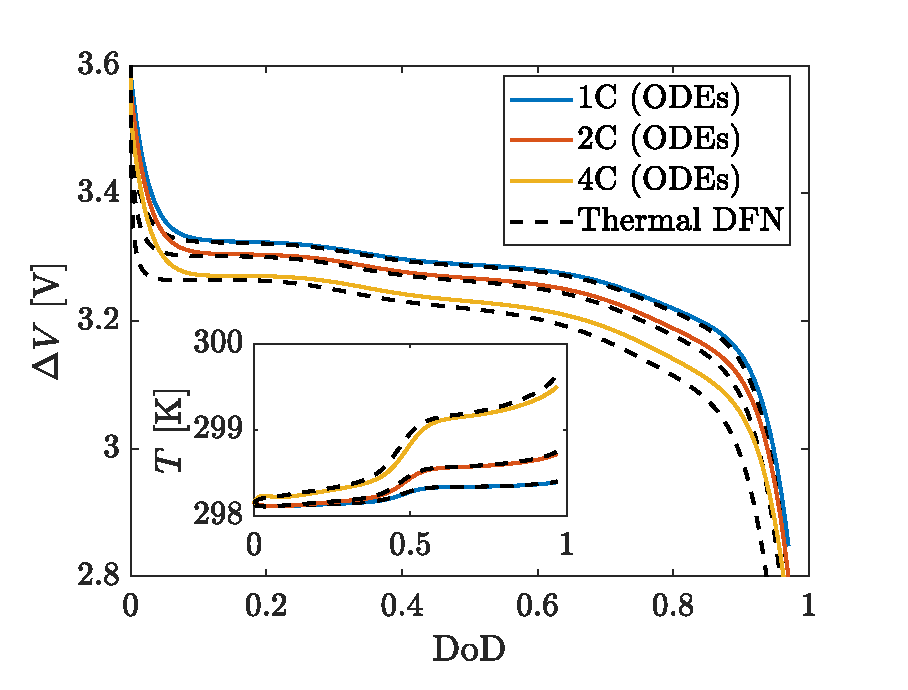
\includegraphics[width=16cm]{figures/V_T_ODEs_DFN}};
	\picbox{images/portraits/hennessy_photo.jpeg}{matt_fast}{lifp_start -| fast_results.east}{north east}
	% Arrows
	\draw [results_arrow] (DFNfast) -- (DFNfast -| fast_results.east);
	\draw [results_arrow] (SPMefast) -- (SPMefast -| fast_results.east);
	\draw [results_arrow] (SPMfast) -- (SPMfast -| fast_results.east);

	%%%%%%%%%%%%%%%%%%%%%%%%%%%%%%%%%%%%%%%%%%%%%%%%%%%%%%%%%%%%%%%%%%%%%%%%%%%%%%%%%%%%%%
	%%%%%%%%%%%%%%%%%%%%%%%%%%%%%%%%%%%%%%%%%%%%%%%%%%%%%%%%%%%%%%%%%%%%%%%%%%%%%%%%%%%%%%
	%%%%%%%%%%%%%%%%%%%%%%%%%%%%%%%%%%%%%%%%%%%%%%%%%%%%%%%%%%%%%%%%%%%%%%%%%%%%%%%%%%%%%%
	% macroscale axis
	% \node [above right = 0cm and 2.5cm of 2plus1D](y_axis_start) {};
	% \node [below right = 0cm and 2.5cm of 0D_macro](y_axis_end) {};
	\node (y_axis_end) at (distributed_results.south -| axis_origin) {};
	\draw [axisline, macrocolor] (axis_origin) -- (y_axis_end)
		node [left, pos=0, rotate=90, anchor=south east] {Complex}
		node [left, pos=0.5, rotate=90, anchor=south] {\Large \textsc{Macroscale}}
		node [below, rotate=90, anchor=south west] {Simple};
\end{tikzpicture}

\end{document}
